\documentclass[]{article}
\usepackage{lmodern}
\usepackage{amssymb,amsmath}
\usepackage{ifxetex,ifluatex}
\usepackage{fixltx2e} % provides \textsubscript
\ifnum 0\ifxetex 1\fi\ifluatex 1\fi=0 % if pdftex
  \usepackage[T1]{fontenc}
  \usepackage[utf8]{inputenc}
\else % if luatex or xelatex
  \ifxetex
    \usepackage{mathspec}
  \else
    \usepackage{fontspec}
  \fi
  \defaultfontfeatures{Ligatures=TeX,Scale=MatchLowercase}
\fi
% use upquote if available, for straight quotes in verbatim environments
\IfFileExists{upquote.sty}{\usepackage{upquote}}{}
% use microtype if available
\IfFileExists{microtype.sty}{%
\usepackage{microtype}
\UseMicrotypeSet[protrusion]{basicmath} % disable protrusion for tt fonts
}{}
\usepackage[margin=1in]{geometry}
\usepackage{hyperref}
\hypersetup{unicode=true,
            pdftitle={Tipos de Gr?ficos},
            pdfborder={0 0 0},
            breaklinks=true}
\urlstyle{same}  % don't use monospace font for urls
\usepackage{color}
\usepackage{fancyvrb}
\newcommand{\VerbBar}{|}
\newcommand{\VERB}{\Verb[commandchars=\\\{\}]}
\DefineVerbatimEnvironment{Highlighting}{Verbatim}{commandchars=\\\{\}}
% Add ',fontsize=\small' for more characters per line
\usepackage{framed}
\definecolor{shadecolor}{RGB}{248,248,248}
\newenvironment{Shaded}{\begin{snugshade}}{\end{snugshade}}
\newcommand{\AlertTok}[1]{\textcolor[rgb]{0.94,0.16,0.16}{#1}}
\newcommand{\AnnotationTok}[1]{\textcolor[rgb]{0.56,0.35,0.01}{\textbf{\textit{#1}}}}
\newcommand{\AttributeTok}[1]{\textcolor[rgb]{0.77,0.63,0.00}{#1}}
\newcommand{\BaseNTok}[1]{\textcolor[rgb]{0.00,0.00,0.81}{#1}}
\newcommand{\BuiltInTok}[1]{#1}
\newcommand{\CharTok}[1]{\textcolor[rgb]{0.31,0.60,0.02}{#1}}
\newcommand{\CommentTok}[1]{\textcolor[rgb]{0.56,0.35,0.01}{\textit{#1}}}
\newcommand{\CommentVarTok}[1]{\textcolor[rgb]{0.56,0.35,0.01}{\textbf{\textit{#1}}}}
\newcommand{\ConstantTok}[1]{\textcolor[rgb]{0.00,0.00,0.00}{#1}}
\newcommand{\ControlFlowTok}[1]{\textcolor[rgb]{0.13,0.29,0.53}{\textbf{#1}}}
\newcommand{\DataTypeTok}[1]{\textcolor[rgb]{0.13,0.29,0.53}{#1}}
\newcommand{\DecValTok}[1]{\textcolor[rgb]{0.00,0.00,0.81}{#1}}
\newcommand{\DocumentationTok}[1]{\textcolor[rgb]{0.56,0.35,0.01}{\textbf{\textit{#1}}}}
\newcommand{\ErrorTok}[1]{\textcolor[rgb]{0.64,0.00,0.00}{\textbf{#1}}}
\newcommand{\ExtensionTok}[1]{#1}
\newcommand{\FloatTok}[1]{\textcolor[rgb]{0.00,0.00,0.81}{#1}}
\newcommand{\FunctionTok}[1]{\textcolor[rgb]{0.00,0.00,0.00}{#1}}
\newcommand{\ImportTok}[1]{#1}
\newcommand{\InformationTok}[1]{\textcolor[rgb]{0.56,0.35,0.01}{\textbf{\textit{#1}}}}
\newcommand{\KeywordTok}[1]{\textcolor[rgb]{0.13,0.29,0.53}{\textbf{#1}}}
\newcommand{\NormalTok}[1]{#1}
\newcommand{\OperatorTok}[1]{\textcolor[rgb]{0.81,0.36,0.00}{\textbf{#1}}}
\newcommand{\OtherTok}[1]{\textcolor[rgb]{0.56,0.35,0.01}{#1}}
\newcommand{\PreprocessorTok}[1]{\textcolor[rgb]{0.56,0.35,0.01}{\textit{#1}}}
\newcommand{\RegionMarkerTok}[1]{#1}
\newcommand{\SpecialCharTok}[1]{\textcolor[rgb]{0.00,0.00,0.00}{#1}}
\newcommand{\SpecialStringTok}[1]{\textcolor[rgb]{0.31,0.60,0.02}{#1}}
\newcommand{\StringTok}[1]{\textcolor[rgb]{0.31,0.60,0.02}{#1}}
\newcommand{\VariableTok}[1]{\textcolor[rgb]{0.00,0.00,0.00}{#1}}
\newcommand{\VerbatimStringTok}[1]{\textcolor[rgb]{0.31,0.60,0.02}{#1}}
\newcommand{\WarningTok}[1]{\textcolor[rgb]{0.56,0.35,0.01}{\textbf{\textit{#1}}}}
\usepackage{graphicx,grffile}
\makeatletter
\def\maxwidth{\ifdim\Gin@nat@width>\linewidth\linewidth\else\Gin@nat@width\fi}
\def\maxheight{\ifdim\Gin@nat@height>\textheight\textheight\else\Gin@nat@height\fi}
\makeatother
% Scale images if necessary, so that they will not overflow the page
% margins by default, and it is still possible to overwrite the defaults
% using explicit options in \includegraphics[width, height, ...]{}
\setkeys{Gin}{width=\maxwidth,height=\maxheight,keepaspectratio}
\IfFileExists{parskip.sty}{%
\usepackage{parskip}
}{% else
\setlength{\parindent}{0pt}
\setlength{\parskip}{6pt plus 2pt minus 1pt}
}
\setlength{\emergencystretch}{3em}  % prevent overfull lines
\providecommand{\tightlist}{%
  \setlength{\itemsep}{0pt}\setlength{\parskip}{0pt}}
\setcounter{secnumdepth}{0}
% Redefines (sub)paragraphs to behave more like sections
\ifx\paragraph\undefined\else
\let\oldparagraph\paragraph
\renewcommand{\paragraph}[1]{\oldparagraph{#1}\mbox{}}
\fi
\ifx\subparagraph\undefined\else
\let\oldsubparagraph\subparagraph
\renewcommand{\subparagraph}[1]{\oldsubparagraph{#1}\mbox{}}
\fi

%%% Use protect on footnotes to avoid problems with footnotes in titles
\let\rmarkdownfootnote\footnote%
\def\footnote{\protect\rmarkdownfootnote}

%%% Change title format to be more compact
\usepackage{titling}

% Create subtitle command for use in maketitle
\providecommand{\subtitle}[1]{
  \posttitle{
    \begin{center}\large#1\end{center}
    }
}

\setlength{\droptitle}{-2em}

  \title{Tipos de Gr?ficos}
    \pretitle{\vspace{\droptitle}\centering\huge}
  \posttitle{\par}
    \author{}
    \preauthor{}\postauthor{}
    \date{}
    \predate{}\postdate{}
  

\begin{document}
\maketitle

\hypertarget{ggplot2}{%
\section{ggplot2}\label{ggplot2}}

A maneira mais fácil de obter o ggplot2 ? instalar o pacote tidyverse O
tidyverse ? uma cole??o de pacotes R projetados para ci?ncia de dados

\begin{Shaded}
\begin{Highlighting}[]
\CommentTok{# install.packages("tidyverse")}
\end{Highlighting}
\end{Shaded}

Como alternativa, instale apenas o ggplot2:

\begin{Shaded}
\begin{Highlighting}[]
\CommentTok{# install.packages("ggplot2")}
\end{Highlighting}
\end{Shaded}

\begin{Shaded}
\begin{Highlighting}[]
\CommentTok{# Carrega o ggplot2}
\KeywordTok{library}\NormalTok{(ggplot2)}
\end{Highlighting}
\end{Shaded}

\hypertarget{grafico-de-barras}{%
\subsubsection{Gráfico de Barras}\label{grafico-de-barras}}


\includegraphics{img/barchart.png}

\begin{Shaded}
\begin{Highlighting}[]
\KeywordTok{plot}\NormalTok{(cars)}
\end{Highlighting}
\end{Shaded}

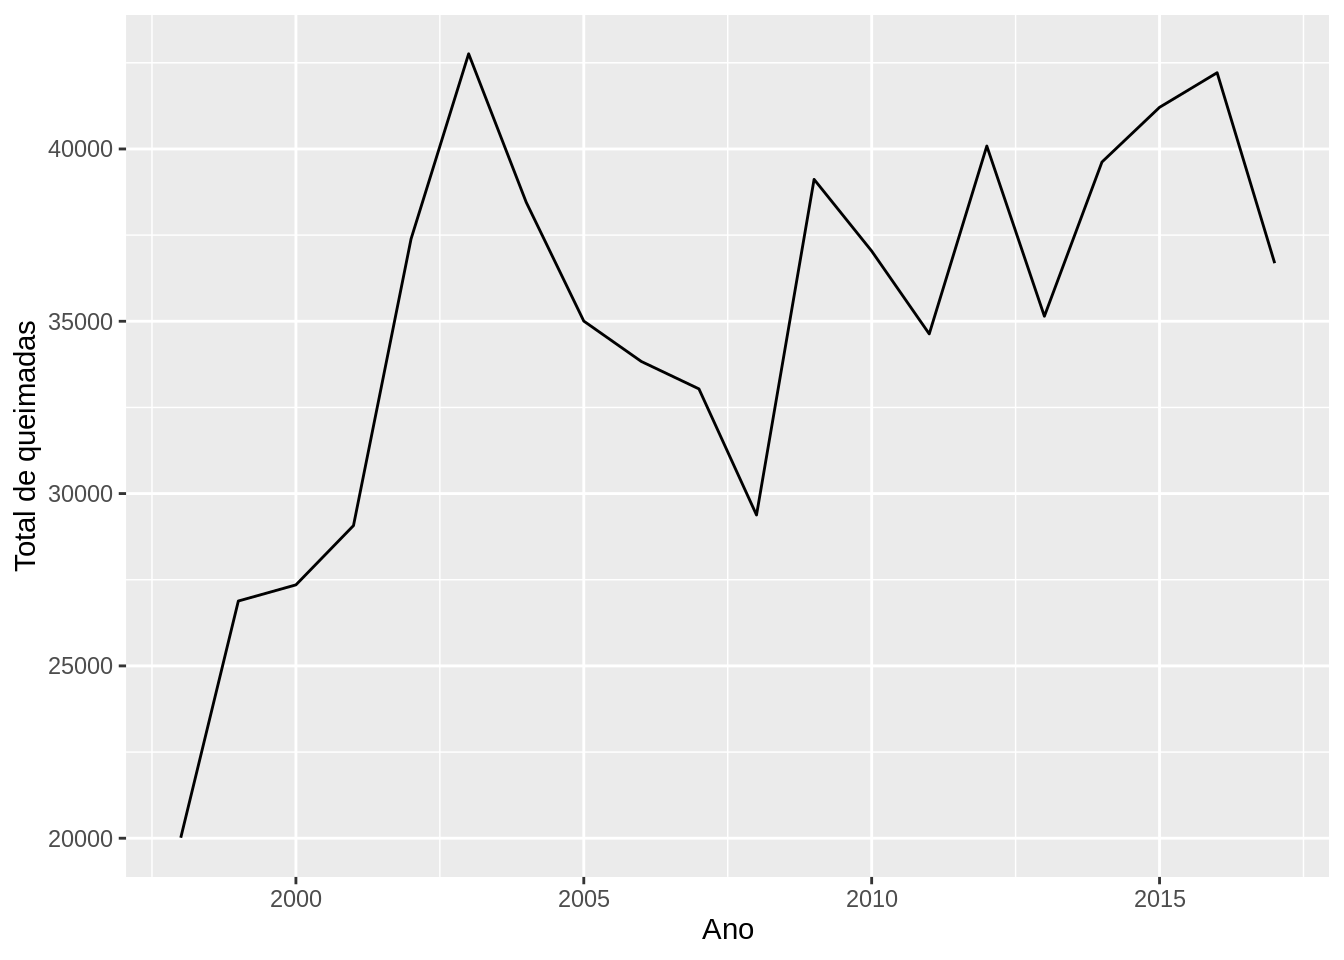
\includegraphics{2_graficos_files/figure-latex/unnamed-chunk-4-1.pdf}

\hypertarget{grfico-de-barras-horizontal}{%
\subsubsection{Gr?fico de Barras
Horizontal}\label{grfico-de-barras-horizontal}}


\includegraphics{img/horizontal_barchart.png}

\hypertarget{histograma}{%
\subsubsection{Histograma}\label{histograma}}


\includegraphics{img/histograma.png}

\hypertarget{grafico-de-dispersao}{%
\subsubsection{Gráfico de Dispersão}\label{grafico-de-dispersao}}


\includegraphics{img/scatterplot.png}

\hypertarget{mapa-de-calor-heatmap}{%
\subsubsection{Mapa de Calor (Heatmap)}\label{mapa-de-calor-heatmap}}


\includegraphics{img/heatmap.png}

\hypertarget{grfico-de-linhas}{%
\subsubsection{Gr?fico de Linhas}\label{grfico-de-linhas}}


\includegraphics{img/line_chart.png}

\hypertarget{grfico-de-rea}{%
\subsubsection{Gr?fico de ?rea}\label{grfico-de-rea}}


\includegraphics{img/area_chart.png}

\hypertarget{grfico-de-rea-empilhada}{%
\subsubsection{Gr?fico de ?rea
Empilhada}\label{grfico-de-rea-empilhada}}


\includegraphics{img/stacked_area.png}

\hypertarget{grfico-de-barras-empilhadas}{%
\subsubsection{Gr?fico de Barras
Empilhadas}\label{grfico-de-barras-empilhadas}}


\includegraphics{img/stacked_bar_chart.png}

\hypertarget{grfico-de-barras-agrupadas}{%
\subsubsection{Gr?fico de Barras
Agrupadas}\label{grfico-de-barras-agrupadas}}


\includegraphics{img/grouped_bar.png}

\hypertarget{grfico-de-setores-pizza}{%
\subsubsection{Gr?fico de Setores
(Pizza)}\label{grfico-de-setores-pizza}}


\includegraphics{img/pie_chart.png}

\hypertarget{grfico-de-setores-rosca}{%
\subsubsection{Gr?fico de Setores
(Rosca)}\label{grfico-de-setores-rosca}}


\includegraphics{img/donut.png}

\hypertarget{treemap}{%
\subsubsection{Treemap}\label{treemap}}


\includegraphics{img/treemap.png}

\hypertarget{referncias}{%
\section{Refer?ncias}\label{referncias}}

\href{https://www.curso-r.com/material/ggplot/}{Gr?ficos com ggplot2}

\href{https://www.r-graph-gallery.com/index.html}{The R Graph Gallery}

\href{http://moderngraphics11.pbworks.com/f/ggplot2-Book09hWickham.pdf}{Hadley
Wickham - ggplot: Elegant graphics for data analysis.}

\href{https://combine-australia.github.io/r-novice-gapminder/ggplot.pdf}{Data
Visualization Using R \& ggplot - Karthik Ram.}

\href{https://www.data-action-lab.com/wp-content/uploads/2018/11/DSRS_GGP2.pdf}{A
ggplot2 Primer.}

\href{http://userweb.eng.gla.ac.uk/umer.ijaz/bioinformatics/ecological/ggplot2.pdf}{ggplot2:
Introduction and exercises - Umer Zeeshan Ijaz.}

\href{https://github.com/ucb-stat133/stat133-fall-2016/blob/master/notes/09-ggplot2/09-ggplot2.pdf}{Getting
started with ggplot2 - Gaston Sanchez.}

\href{https://journalismcourses.org/courses/RC0818/charts_with_ggplot.pdf}{Charts
with ggplot2 -Andrew Ba Tran.}

\href{http://www.math.montana.edu/ahoegh/teaching/stat408/lecturematerials/}{STAT
408.}

\href{https://github.com/hadley/ggplot2-book}{ggplot2: elegant graphics
for data analysis}


\end{document}
